% Options for packages loaded elsewhere
% Options for packages loaded elsewhere
\PassOptionsToPackage{unicode}{hyperref}
\PassOptionsToPackage{hyphens}{url}
\PassOptionsToPackage{dvipsnames,svgnames,x11names}{xcolor}
%
\documentclass[
  russian,
  letterpaper,
  DIV=11,
  numbers=noendperiod,
  oneside]{scrreprt}
\usepackage{xcolor}
\usepackage[left=1in,marginparwidth=2.0666666666667in,textwidth=4.1333333333333in,marginparsep=0.3in]{geometry}
\usepackage{amsmath,amssymb}
\setcounter{secnumdepth}{5}
\usepackage{iftex}
\ifPDFTeX
  \usepackage[T1]{fontenc}
  \usepackage[utf8]{inputenc}
  \usepackage{textcomp} % provide euro and other symbols
\else % if luatex or xetex
  \usepackage{unicode-math} % this also loads fontspec
  \defaultfontfeatures{Scale=MatchLowercase}
  \defaultfontfeatures[\rmfamily]{Ligatures=TeX,Scale=1}
\fi
\usepackage{lmodern}
\ifPDFTeX\else
  % xetex/luatex font selection
\fi
% Use upquote if available, for straight quotes in verbatim environments
\IfFileExists{upquote.sty}{\usepackage{upquote}}{}
\IfFileExists{microtype.sty}{% use microtype if available
  \usepackage[]{microtype}
  \UseMicrotypeSet[protrusion]{basicmath} % disable protrusion for tt fonts
}{}
\makeatletter
\@ifundefined{KOMAClassName}{% if non-KOMA class
  \IfFileExists{parskip.sty}{%
    \usepackage{parskip}
  }{% else
    \setlength{\parindent}{0pt}
    \setlength{\parskip}{6pt plus 2pt minus 1pt}}
}{% if KOMA class
  \KOMAoptions{parskip=half}}
\makeatother
% Make \paragraph and \subparagraph free-standing
\makeatletter
\ifx\paragraph\undefined\else
  \let\oldparagraph\paragraph
  \renewcommand{\paragraph}{
    \@ifstar
      \xxxParagraphStar
      \xxxParagraphNoStar
  }
  \newcommand{\xxxParagraphStar}[1]{\oldparagraph*{#1}\mbox{}}
  \newcommand{\xxxParagraphNoStar}[1]{\oldparagraph{#1}\mbox{}}
\fi
\ifx\subparagraph\undefined\else
  \let\oldsubparagraph\subparagraph
  \renewcommand{\subparagraph}{
    \@ifstar
      \xxxSubParagraphStar
      \xxxSubParagraphNoStar
  }
  \newcommand{\xxxSubParagraphStar}[1]{\oldsubparagraph*{#1}\mbox{}}
  \newcommand{\xxxSubParagraphNoStar}[1]{\oldsubparagraph{#1}\mbox{}}
\fi
\makeatother

\usepackage{color}
\usepackage{fancyvrb}
\newcommand{\VerbBar}{|}
\newcommand{\VERB}{\Verb[commandchars=\\\{\}]}
\DefineVerbatimEnvironment{Highlighting}{Verbatim}{commandchars=\\\{\}}
% Add ',fontsize=\small' for more characters per line
\usepackage{framed}
\definecolor{shadecolor}{RGB}{241,243,245}
\newenvironment{Shaded}{\begin{snugshade}}{\end{snugshade}}
\newcommand{\AlertTok}[1]{\textcolor[rgb]{0.68,0.00,0.00}{#1}}
\newcommand{\AnnotationTok}[1]{\textcolor[rgb]{0.37,0.37,0.37}{#1}}
\newcommand{\AttributeTok}[1]{\textcolor[rgb]{0.40,0.45,0.13}{#1}}
\newcommand{\BaseNTok}[1]{\textcolor[rgb]{0.68,0.00,0.00}{#1}}
\newcommand{\BuiltInTok}[1]{\textcolor[rgb]{0.00,0.23,0.31}{#1}}
\newcommand{\CharTok}[1]{\textcolor[rgb]{0.13,0.47,0.30}{#1}}
\newcommand{\CommentTok}[1]{\textcolor[rgb]{0.37,0.37,0.37}{#1}}
\newcommand{\CommentVarTok}[1]{\textcolor[rgb]{0.37,0.37,0.37}{\textit{#1}}}
\newcommand{\ConstantTok}[1]{\textcolor[rgb]{0.56,0.35,0.01}{#1}}
\newcommand{\ControlFlowTok}[1]{\textcolor[rgb]{0.00,0.23,0.31}{\textbf{#1}}}
\newcommand{\DataTypeTok}[1]{\textcolor[rgb]{0.68,0.00,0.00}{#1}}
\newcommand{\DecValTok}[1]{\textcolor[rgb]{0.68,0.00,0.00}{#1}}
\newcommand{\DocumentationTok}[1]{\textcolor[rgb]{0.37,0.37,0.37}{\textit{#1}}}
\newcommand{\ErrorTok}[1]{\textcolor[rgb]{0.68,0.00,0.00}{#1}}
\newcommand{\ExtensionTok}[1]{\textcolor[rgb]{0.00,0.23,0.31}{#1}}
\newcommand{\FloatTok}[1]{\textcolor[rgb]{0.68,0.00,0.00}{#1}}
\newcommand{\FunctionTok}[1]{\textcolor[rgb]{0.28,0.35,0.67}{#1}}
\newcommand{\ImportTok}[1]{\textcolor[rgb]{0.00,0.46,0.62}{#1}}
\newcommand{\InformationTok}[1]{\textcolor[rgb]{0.37,0.37,0.37}{#1}}
\newcommand{\KeywordTok}[1]{\textcolor[rgb]{0.00,0.23,0.31}{\textbf{#1}}}
\newcommand{\NormalTok}[1]{\textcolor[rgb]{0.00,0.23,0.31}{#1}}
\newcommand{\OperatorTok}[1]{\textcolor[rgb]{0.37,0.37,0.37}{#1}}
\newcommand{\OtherTok}[1]{\textcolor[rgb]{0.00,0.23,0.31}{#1}}
\newcommand{\PreprocessorTok}[1]{\textcolor[rgb]{0.68,0.00,0.00}{#1}}
\newcommand{\RegionMarkerTok}[1]{\textcolor[rgb]{0.00,0.23,0.31}{#1}}
\newcommand{\SpecialCharTok}[1]{\textcolor[rgb]{0.37,0.37,0.37}{#1}}
\newcommand{\SpecialStringTok}[1]{\textcolor[rgb]{0.13,0.47,0.30}{#1}}
\newcommand{\StringTok}[1]{\textcolor[rgb]{0.13,0.47,0.30}{#1}}
\newcommand{\VariableTok}[1]{\textcolor[rgb]{0.07,0.07,0.07}{#1}}
\newcommand{\VerbatimStringTok}[1]{\textcolor[rgb]{0.13,0.47,0.30}{#1}}
\newcommand{\WarningTok}[1]{\textcolor[rgb]{0.37,0.37,0.37}{\textit{#1}}}

\usepackage{longtable,booktabs,array}
\usepackage{calc} % for calculating minipage widths
% Correct order of tables after \paragraph or \subparagraph
\usepackage{etoolbox}
\makeatletter
\patchcmd\longtable{\par}{\if@noskipsec\mbox{}\fi\par}{}{}
\makeatother
% Allow footnotes in longtable head/foot
\IfFileExists{footnotehyper.sty}{\usepackage{footnotehyper}}{\usepackage{footnote}}
\makesavenoteenv{longtable}
\usepackage{graphicx}
\makeatletter
\newsavebox\pandoc@box
\newcommand*\pandocbounded[1]{% scales image to fit in text height/width
  \sbox\pandoc@box{#1}%
  \Gscale@div\@tempa{\textheight}{\dimexpr\ht\pandoc@box+\dp\pandoc@box\relax}%
  \Gscale@div\@tempb{\linewidth}{\wd\pandoc@box}%
  \ifdim\@tempb\p@<\@tempa\p@\let\@tempa\@tempb\fi% select the smaller of both
  \ifdim\@tempa\p@<\p@\scalebox{\@tempa}{\usebox\pandoc@box}%
  \else\usebox{\pandoc@box}%
  \fi%
}
% Set default figure placement to htbp
\def\fps@figure{htbp}
\makeatother


% definitions for citeproc citations
\NewDocumentCommand\citeproctext{}{}
\NewDocumentCommand\citeproc{mm}{%
  \begingroup\def\citeproctext{#2}\cite{#1}\endgroup}
\makeatletter
 % allow citations to break across lines
 \let\@cite@ofmt\@firstofone
 % avoid brackets around text for \cite:
 \def\@biblabel#1{}
 \def\@cite#1#2{{#1\if@tempswa , #2\fi}}
\makeatother
\newlength{\cslhangindent}
\setlength{\cslhangindent}{1.5em}
\newlength{\csllabelwidth}
\setlength{\csllabelwidth}{3em}
\newenvironment{CSLReferences}[2] % #1 hanging-indent, #2 entry-spacing
 {\begin{list}{}{%
  \setlength{\itemindent}{0pt}
  \setlength{\leftmargin}{0pt}
  \setlength{\parsep}{0pt}
  % turn on hanging indent if param 1 is 1
  \ifodd #1
   \setlength{\leftmargin}{\cslhangindent}
   \setlength{\itemindent}{-1\cslhangindent}
  \fi
  % set entry spacing
  \setlength{\itemsep}{#2\baselineskip}}}
 {\end{list}}
\usepackage{calc}
\newcommand{\CSLBlock}[1]{\hfill\break\parbox[t]{\linewidth}{\strut\ignorespaces#1\strut}}
\newcommand{\CSLLeftMargin}[1]{\parbox[t]{\csllabelwidth}{\strut#1\strut}}
\newcommand{\CSLRightInline}[1]{\parbox[t]{\linewidth - \csllabelwidth}{\strut#1\strut}}
\newcommand{\CSLIndent}[1]{\hspace{\cslhangindent}#1}

\ifLuaTeX
\usepackage[bidi=basic,provide=*]{babel}
\else
\usepackage[bidi=default,provide=*]{babel}
\fi
% get rid of language-specific shorthands (see #6817):
\let\LanguageShortHands\languageshorthands
\def\languageshorthands#1{}


\setlength{\emergencystretch}{3em} % prevent overfull lines

\providecommand{\tightlist}{%
  \setlength{\itemsep}{0pt}\setlength{\parskip}{0pt}}



 


\KOMAoption{captions}{tableheading}
\makeatletter
\@ifpackageloaded{tcolorbox}{}{\usepackage[skins,breakable]{tcolorbox}}
\@ifpackageloaded{fontawesome5}{}{\usepackage{fontawesome5}}
\definecolor{quarto-callout-color}{HTML}{909090}
\definecolor{quarto-callout-note-color}{HTML}{0758E5}
\definecolor{quarto-callout-important-color}{HTML}{CC1914}
\definecolor{quarto-callout-warning-color}{HTML}{EB9113}
\definecolor{quarto-callout-tip-color}{HTML}{00A047}
\definecolor{quarto-callout-caution-color}{HTML}{FC5300}
\definecolor{quarto-callout-color-frame}{HTML}{acacac}
\definecolor{quarto-callout-note-color-frame}{HTML}{4582ec}
\definecolor{quarto-callout-important-color-frame}{HTML}{d9534f}
\definecolor{quarto-callout-warning-color-frame}{HTML}{f0ad4e}
\definecolor{quarto-callout-tip-color-frame}{HTML}{02b875}
\definecolor{quarto-callout-caution-color-frame}{HTML}{fd7e14}
\makeatother
\makeatletter
\@ifpackageloaded{bookmark}{}{\usepackage{bookmark}}
\makeatother
\makeatletter
\@ifpackageloaded{caption}{}{\usepackage{caption}}
\AtBeginDocument{%
\ifdefined\contentsname
  \renewcommand*\contentsname{Содержание}
\else
  \newcommand\contentsname{Содержание}
\fi
\ifdefined\listfigurename
  \renewcommand*\listfigurename{Список Иллюстраций}
\else
  \newcommand\listfigurename{Список Иллюстраций}
\fi
\ifdefined\listtablename
  \renewcommand*\listtablename{Список Таблиц}
\else
  \newcommand\listtablename{Список Таблиц}
\fi
\ifdefined\figurename
  \renewcommand*\figurename{Рисунок}
\else
  \newcommand\figurename{Рисунок}
\fi
\ifdefined\tablename
  \renewcommand*\tablename{Таблица}
\else
  \newcommand\tablename{Таблица}
\fi
}
\@ifpackageloaded{float}{}{\usepackage{float}}
\floatstyle{ruled}
\@ifundefined{c@chapter}{\newfloat{codelisting}{h}{lop}}{\newfloat{codelisting}{h}{lop}[chapter]}
\floatname{codelisting}{Список}
\newcommand*\listoflistings{\listof{codelisting}{Список Каталогов}}
\usepackage{amsthm}
\theoremstyle{definition}
\newtheorem{exercise}{Упражнение}[chapter]
\theoremstyle{plain}
\newtheorem{proposition}{Утверждение}[chapter]
\theoremstyle{plain}
\newtheorem{lemma}{Лемма}[chapter]
\theoremstyle{definition}
\newtheorem{definition}{Определение}[chapter]
\theoremstyle{plain}
\newtheorem{theorem}{Теорема}[chapter]
\theoremstyle{plain}
\newtheorem{conjecture}{Гипотеза}[chapter]
\theoremstyle{plain}
\newtheorem{corollary}{Следствие}[chapter]
\theoremstyle{plain}
\newtheorem{algorithm}{Algorithm}[chapter]
\theoremstyle{definition}
\newtheorem{example}{Пример}[chapter]
\theoremstyle{remark}
\AtBeginDocument{\renewcommand*{\proofname}{Доказательство}}
\newtheorem*{remark}{Примечание}
\newtheorem*{solution}{Решение}
\newtheorem{refremark}{Примечание}[chapter]
\newtheorem{refsolution}{Решение}[chapter]
\makeatother
\makeatletter
\makeatother
\makeatletter
\@ifpackageloaded{caption}{}{\usepackage{caption}}
\@ifpackageloaded{subcaption}{}{\usepackage{subcaption}}
\makeatother
\makeatletter
\@ifpackageloaded{sidenotes}{}{\usepackage{sidenotes}}
\@ifpackageloaded{marginnote}{}{\usepackage{marginnote}}
\makeatother
\makeatletter
\@ifpackageloaded{tikz}{}{\usepackage{tikz}}
\makeatother
        \newcommand*\circled[1]{\tikz[baseline=(char.base)]{
          \node[shape=circle,draw,inner sep=1pt] (char) {{\scriptsize#1}};}}  
                  
\newcounter{quartocalloutnteno}
\newcommand{\quartocalloutnte}[1]{\refstepcounter{quartocalloutnteno}\label{#1}}
\newcounter{quartocallouttipno}
\newcommand{\quartocallouttip}[1]{\refstepcounter{quartocallouttipno}\label{#1}}
\newcounter{quartocalloutwrnno}
\newcommand{\quartocalloutwrn}[1]{\refstepcounter{quartocalloutwrnno}\label{#1}}
\newcounter{quartocalloutcauno}
\newcommand{\quartocalloutcau}[1]{\refstepcounter{quartocalloutcauno}\label{#1}}
\newcounter{quartocalloutimpno}
\newcommand{\quartocalloutimp}[1]{\refstepcounter{quartocalloutimpno}\label{#1}}
\usepackage{bookmark}
\IfFileExists{xurl.sty}{\usepackage{xurl}}{} % add URL line breaks if available
\urlstyle{same}
\hypersetup{
  pdftitle={WLM~SDARP},
  pdfauthor={Антон Ангельгардт},
  pdflang={ru},
  colorlinks=true,
  linkcolor={blue},
  filecolor={Maroon},
  citecolor={Blue},
  urlcolor={Blue},
  pdfcreator={LaTeX via pandoc}}


\title{WLM~SDARP}
\usepackage{etoolbox}
\makeatletter
\providecommand{\subtitle}[1]{% add subtitle to \maketitle
  \apptocmd{\@title}{\par {\large #1 \par}}{}{}
}
\makeatother
\subtitle{Мир линейных моделей: статистика и~анализ данных в~R
для~психологов}
\author{Антон Ангельгардт}
\date{2026-04-13}
\begin{document}
\maketitle

\renewcommand*\contentsname{Содержание}
{
\hypersetup{linkcolor=}
\setcounter{tocdepth}{2}
\tableofcontents
}

\bookmarksetup{startatroot}

\chapter{Cover Page}\label{cover-page}

\part{Часть {[}отладка{]}}

Титульная страница части.

Значимость этих проблем крайне не ясна, что укрепление и развитие
структуры представляет собой интересный эксперимент проверки системы
обучения кадров, соответствует насущным потребностям. Идейные
соображения высшего порядка, а также дальнейшее развитие различных форм
деятельности способствует подготовки и реализации существенных
финансовых и административных условий.

Ещё абзац.

\chapter{Глава
{[}отладка{]}}\label{ux433ux43bux430ux432ux430-ux43eux442ux43bux430ux434ux43aux430}

\newcommand{\circled}[1]{\enclose{circle}{#1}}

\newcommand{\const}{\text{const}}
\newcommand{\fix}{\text{fix}}
\DeclareMathOperator{\sgn}{sgn}
\newcommand{\lp}{\left(}
\newcommand{\rp}{\right)}
\newcommand{\lb}{\left[}
\newcommand{\rb}{\right]}

\newcommand{\defin}[1]{\overset{\text{def}}{#1}}
\newcommand{\toas}{\overset{\text{a.s.}}{\to}}
\newcommand{\toprob}{\overset{p}{\to}}
\newcommand{\todist}{\overset{d}{\to}}

\newcommand{\true}{\mathsf{T}}
\newcommand{\false}{\mathsf{F}}

---\textgreater{}

Текст введения.

Значимость этих проблем крайне не ясна, что укрепление и развитие
структуры представляет собой интересный эксперимент проверки системы
обучения кадров, соответствует насущным потребностям.

Идейные соображения высшего порядка, а также дальнейшее развитие
различных форм деятельности способствует подгото вки и реализации
существенных финансовых и административных условий.

\section{Текст}\label{debug-text}

Значимость этих проблем крайне не ясна, что укрепление и развитие
структуры представляет собой интересный эксперимент проверки системы
обучения кадров, соответствует насущным потребностям.

Идейные соображения высшего порядка, а также дальнейшее развитие
различных форм деятельности способствует подгото вки и реализации
существенных финансовых и административных условий (Knuth 1984).

\begin{quote}
Это цитата, оформленная средствами Markdown из~коробки.
\end{quote}

\section{Лейблы}\label{debug-labs}

Просто тестовый текст.

\subsection{Раздел для~нешарящих}\label{debug-labs-novice}

Разнообразный и богатый опыт постоянное информационно-пропагандистское
обеспечение нашей деятельности требуют определения и уточнения позиций,
занимаемых участниками в отношении поставленных задач. Идейные
соображения высшего порядка, а также реализация намеченных плановых
заданий в значительной степени обуславливает создание направлений
прогрессивного развития.

\subsection{Раздел для~чуть шарящих}\label{debug-labs-junior}

С другой стороны начало повседневной работы по формированию позиции
влечет за собой процесс внедрения и модернизации позиций, занимаемых
участниками в отношении поставленных задач.

\subsection{Раздел для~ шарящих}\label{debug-labs-middle}

Товарищи! новая модель организационной деятельности в значительной
степени обуславливает создание позиций, занимаемых участниками в
отношении поставленных задач. Значимость этих проблем настолько
очевидна, что укрепление и развитие структуры способствует подготовки и
реализации направлений прогрессивного развития.

\subsection{Раздел для~нормально шарящих}\label{debug-labs-senior}

Не следует, однако забывать, что начало повседневной работы по
формированию позиции позволяет выполнять важные задания по разработке
модели развития.

\subsection{Раздел для~крайне шарящих с~очень длинным заголовком
о~невероятно важном содержании раздела}\label{debug-labs-expert}

Таким образом новая модель организационной деятельности способствует
подготовки и реализации соответствующий условий активизации.
Повседневная практика показывает, что постоянный количественный рост и
сфера нашей активности требуют от нас анализа систем массового участия.

\section{Layout}\label{debug-layout}

Здесь даны базовые лэйауты. Больше инфы см.
\url{https://quarto.org/docs/authoring/article-layout.html}.

Для чанков есть cell option \texttt{\#\textbar{}\ column:\ screen}.

\begin{figure}[H]

{\centering \pandocbounded{
\includegraphics[keepaspectratio]{chapters/ru/_debug/img/debug-pic.jpg}}

}

\caption{Дебажная картина. .column-body (дефолт)}

\end{figure}%

\begin{figure}[H]

{\centering \pandocbounded{
\includegraphics[keepaspectratio]{chapters/ru/_debug/img/debug-pic.jpg}}

}

\caption{Дебажная картина. .column-body-outset}

\end{figure}%

\begin{figure*}

\begin{figure}[H]

{\centering \pandocbounded{
\includegraphics[keepaspectratio]{chapters/ru/_debug/img/debug-pic.jpg}}

}

\caption{Дебажная картина. .column-page}

\end{figure}%

\end{figure*}%

\begin{figure*}

\begin{figure}[H]

{\centering \pandocbounded{
\includegraphics[keepaspectratio]{chapters/ru/_debug/img/debug-pic.jpg}}

}

\caption{Дебажная картина. .column-page-inset}

\end{figure}%

\end{figure*}%

\begin{figure*}

\begin{figure}[H]

{\centering \pandocbounded{
\includegraphics[keepaspectratio]{chapters/ru/_debug/img/debug-pic.jpg}}

}

\caption{Дебажная картина. .column-screen}

\end{figure}%

\end{figure*}%

\begin{figure*}

\begin{figure}[H]

{\centering \pandocbounded{
\includegraphics[keepaspectratio]{chapters/ru/_debug/img/debug-pic.jpg}}

}

\caption{Дебажная картина. .column-screen-inset}

\end{figure}%

\end{figure*}%

\marginnote{\begin{footnotesize}

\begin{figure}[H]

{\centering \pandocbounded{
\includegraphics[keepaspectratio]{chapters/ru/_debug/img/debug-pic.jpg}}

}

\caption{Дебажная картина. .column-margin}

\end{figure}%

\end{footnotesize}}

\section{Callouts}\label{debug-callout}

Это текст для~отсмотра кроссреф-ссылок на:

\begin{itemize}
\tightlist
\item
  Note~\ref{nte-debug-id}
\item
  Tip~\ref{tip-debug-id}
\item
  Caution~\ref{cau-debug-id}
\item
  Warning~\ref{wrn-debug-id}
\item
  Important~\ref{imp-debug-id}
\item
  Note~\ref{nte-debug-title-id}
\item
  Tip~\ref{tip-debug-title-id}
\item
  Caution~\ref{cau-debug-title-id}
\item
  Warning~\ref{wrn-debug-title-id}
\item
  Important~\ref{imp-debug-title-id}
\end{itemize}

\subsection{Notes}\label{debug-callout-note}

\begin{tcolorbox}[enhanced jigsaw, opacitybacktitle=0.6, toptitle=1mm, bottomtitle=1mm, leftrule=.75mm, breakable, arc=.35mm, colback=white, title=\textcolor{quarto-callout-note-color}{\faInfo}\hspace{0.5em}{Уведомление}, rightrule=.15mm, opacityback=0, coltitle=black, left=2mm, bottomrule=.15mm, colframe=quarto-callout-note-color-frame, colbacktitle=quarto-callout-note-color!10!white, titlerule=0mm, toprule=.15mm]

Это заметка без~заголовка и~без~id.

\end{tcolorbox}

\begin{tcolorbox}[enhanced jigsaw, opacitybacktitle=0.6, toptitle=1mm, bottomtitle=1mm, leftrule=.75mm, breakable, arc=.35mm, colback=white, title=\textcolor{quarto-callout-note-color}{\faInfo}\hspace{0.5em}{Уведомление \ref*{nte-debug-id}}, rightrule=.15mm, opacityback=0, coltitle=black, left=2mm, bottomrule=.15mm, colframe=quarto-callout-note-color-frame, colbacktitle=quarto-callout-note-color!10!white, titlerule=0mm, toprule=.15mm]

\quartocalloutnte{nte-debug-id} 

Это заметка без~заголовка, но~с~id.

\end{tcolorbox}

\begin{tcolorbox}[enhanced jigsaw, opacitybacktitle=0.6, toptitle=1mm, bottomtitle=1mm, leftrule=.75mm, breakable, arc=.35mm, colback=white, title=\textcolor{quarto-callout-note-color}{\faInfo}\hspace{0.5em}{Заголовок заметки}, rightrule=.15mm, opacityback=0, coltitle=black, left=2mm, bottomrule=.15mm, colframe=quarto-callout-note-color-frame, colbacktitle=quarto-callout-note-color!10!white, titlerule=0mm, toprule=.15mm]

Это заметка с~заголовком, но~без~id.

\end{tcolorbox}

\begin{tcolorbox}[enhanced jigsaw, opacitybacktitle=0.6, toptitle=1mm, bottomtitle=1mm, leftrule=.75mm, breakable, arc=.35mm, colback=white, title=\textcolor{quarto-callout-note-color}{\faInfo}\hspace{0.5em}{Уведомление \ref*{nte-debug-title-id}: Заголовок заметки}, rightrule=.15mm, opacityback=0, coltitle=black, left=2mm, bottomrule=.15mm, colframe=quarto-callout-note-color-frame, colbacktitle=quarto-callout-note-color!10!white, titlerule=0mm, toprule=.15mm]

\quartocalloutnte{nte-debug-title-id} 

Это заметка с~заголовком и~с~id.

\end{tcolorbox}

\subsubsection{Стилевые варианты}\label{debug-callout-note-appearance}

\begin{tcolorbox}[enhanced jigsaw, opacitybacktitle=0.6, toptitle=1mm, bottomtitle=1mm, leftrule=.75mm, breakable, arc=.35mm, colback=white, title=\textcolor{quarto-callout-note-color}{\faInfo}\hspace{0.5em}{Заголовок заметки}, rightrule=.15mm, opacityback=0, coltitle=black, left=2mm, bottomrule=.15mm, colframe=quarto-callout-note-color-frame, colbacktitle=quarto-callout-note-color!10!white, titlerule=0mm, toprule=.15mm]

Это развернутая заметка с~заголовком в~дефолтном оформлении.

\end{tcolorbox}

\begin{tcolorbox}[enhanced jigsaw, opacitybacktitle=0.6, toptitle=1mm, bottomtitle=1mm, leftrule=.75mm, breakable, arc=.35mm, colback=white, title=\textcolor{quarto-callout-note-color}{\faInfo}\hspace{0.5em}{Заголовок заметки}, rightrule=.15mm, opacityback=0, coltitle=black, left=2mm, bottomrule=.15mm, colframe=quarto-callout-note-color-frame, colbacktitle=quarto-callout-note-color!10!white, titlerule=0mm, toprule=.15mm]

Это свернутая заметка с~заголовком в~дефолтном оформлении.

\end{tcolorbox}

\begin{tcolorbox}[enhanced jigsaw, rightrule=.15mm, opacityback=0, left=2mm, leftrule=.75mm, breakable, bottomrule=.15mm, colframe=quarto-callout-note-color-frame, arc=.35mm, colback=white, toprule=.15mm]
\begin{minipage}[t]{5.5mm}
\textcolor{quarto-callout-note-color}{\faInfo}
\end{minipage}%
\begin{minipage}[t]{\textwidth - 5.5mm}

\vspace{-3mm}\textbf{Заголовок заметки}\vspace{3mm}

Это развернутая заметка с~заголовком в~простом оформлении.

\end{minipage}%
\end{tcolorbox}

\begin{tcolorbox}[enhanced jigsaw, rightrule=.15mm, opacityback=0, left=2mm, leftrule=.75mm, breakable, bottomrule=.15mm, colframe=quarto-callout-note-color-frame, arc=.35mm, colback=white, toprule=.15mm]
\begin{minipage}[t]{5.5mm}
\textcolor{quarto-callout-note-color}{\faInfo}
\end{minipage}%
\begin{minipage}[t]{\textwidth - 5.5mm}

\vspace{-3mm}\textbf{Заголовок заметки}\vspace{3mm}

Это свернутая заметка с~заголовком в~простом оформлении.

\end{minipage}%
\end{tcolorbox}

\begin{tcolorbox}[enhanced jigsaw, rightrule=.15mm, opacityback=0, left=2mm, leftrule=.75mm, breakable, bottomrule=.15mm, colframe=quarto-callout-note-color-frame, arc=.35mm, colback=white, toprule=.15mm]

\vspace{-3mm}\textbf{Заголовок заметки}\vspace{3mm}

Это развернутая заметка с~заголовком в~минимальном оформлении.

\end{tcolorbox}

\begin{tcolorbox}[enhanced jigsaw, rightrule=.15mm, opacityback=0, left=2mm, leftrule=.75mm, breakable, bottomrule=.15mm, colframe=quarto-callout-note-color-frame, arc=.35mm, colback=white, toprule=.15mm]

\vspace{-3mm}\textbf{Заголовок заметки}\vspace{3mm}

Это свернутая заметка с~заголовком в~минимальном оформлении.

\end{tcolorbox}

\subsection{Tips}\label{debug-callout-tip}

\begin{tcolorbox}[enhanced jigsaw, opacitybacktitle=0.6, toptitle=1mm, bottomtitle=1mm, leftrule=.75mm, breakable, arc=.35mm, colback=white, title=\textcolor{quarto-callout-tip-color}{\faLightbulb}\hspace{0.5em}{Совет}, rightrule=.15mm, opacityback=0, coltitle=black, left=2mm, bottomrule=.15mm, colframe=quarto-callout-tip-color-frame, colbacktitle=quarto-callout-tip-color!10!white, titlerule=0mm, toprule=.15mm]

Это совет без~заголовка и~без~id.

\end{tcolorbox}

\begin{tcolorbox}[enhanced jigsaw, opacitybacktitle=0.6, toptitle=1mm, bottomtitle=1mm, leftrule=.75mm, breakable, arc=.35mm, colback=white, title=\textcolor{quarto-callout-tip-color}{\faLightbulb}\hspace{0.5em}{Совет \ref*{tip-debug-id}}, rightrule=.15mm, opacityback=0, coltitle=black, left=2mm, bottomrule=.15mm, colframe=quarto-callout-tip-color-frame, colbacktitle=quarto-callout-tip-color!10!white, titlerule=0mm, toprule=.15mm]

\quartocallouttip{tip-debug-id} 

Это совет без~заголовка, но~с~id.

\end{tcolorbox}

\begin{tcolorbox}[enhanced jigsaw, opacitybacktitle=0.6, toptitle=1mm, bottomtitle=1mm, leftrule=.75mm, breakable, arc=.35mm, colback=white, title=\textcolor{quarto-callout-tip-color}{\faLightbulb}\hspace{0.5em}{Заголовок совета}, rightrule=.15mm, opacityback=0, coltitle=black, left=2mm, bottomrule=.15mm, colframe=quarto-callout-tip-color-frame, colbacktitle=quarto-callout-tip-color!10!white, titlerule=0mm, toprule=.15mm]

Это совет с~заголовком, но~без~id.

\end{tcolorbox}

\begin{tcolorbox}[enhanced jigsaw, opacitybacktitle=0.6, toptitle=1mm, bottomtitle=1mm, leftrule=.75mm, breakable, arc=.35mm, colback=white, title=\textcolor{quarto-callout-tip-color}{\faLightbulb}\hspace{0.5em}{Совет \ref*{tip-debug-title-id}: Заголовок совета}, rightrule=.15mm, opacityback=0, coltitle=black, left=2mm, bottomrule=.15mm, colframe=quarto-callout-tip-color-frame, colbacktitle=quarto-callout-tip-color!10!white, titlerule=0mm, toprule=.15mm]

\quartocallouttip{tip-debug-title-id} 

Это совет с~заголовком и~с~id.

\end{tcolorbox}

\subsubsection{Стилевые варианты}\label{debug-callout-tip-appearance}

\begin{tcolorbox}[enhanced jigsaw, opacitybacktitle=0.6, toptitle=1mm, bottomtitle=1mm, leftrule=.75mm, breakable, arc=.35mm, colback=white, title=\textcolor{quarto-callout-tip-color}{\faLightbulb}\hspace{0.5em}{Заголовок совета}, rightrule=.15mm, opacityback=0, coltitle=black, left=2mm, bottomrule=.15mm, colframe=quarto-callout-tip-color-frame, colbacktitle=quarto-callout-tip-color!10!white, titlerule=0mm, toprule=.15mm]

Это развернутый совет с~заголовком в~дефолтном оформлении.

\end{tcolorbox}

\begin{tcolorbox}[enhanced jigsaw, opacitybacktitle=0.6, toptitle=1mm, bottomtitle=1mm, leftrule=.75mm, breakable, arc=.35mm, colback=white, title=\textcolor{quarto-callout-tip-color}{\faLightbulb}\hspace{0.5em}{Заголовок совета}, rightrule=.15mm, opacityback=0, coltitle=black, left=2mm, bottomrule=.15mm, colframe=quarto-callout-tip-color-frame, colbacktitle=quarto-callout-tip-color!10!white, titlerule=0mm, toprule=.15mm]

Это свернутый совет с~заголовком в~дефолтном оформлении.

\end{tcolorbox}

\begin{tcolorbox}[enhanced jigsaw, rightrule=.15mm, opacityback=0, left=2mm, leftrule=.75mm, breakable, bottomrule=.15mm, colframe=quarto-callout-tip-color-frame, arc=.35mm, colback=white, toprule=.15mm]
\begin{minipage}[t]{5.5mm}
\textcolor{quarto-callout-tip-color}{\faLightbulb}
\end{minipage}%
\begin{minipage}[t]{\textwidth - 5.5mm}

\vspace{-3mm}\textbf{Заголовок совета}\vspace{3mm}

Это развернутый совет с~заголовком в~простом оформлении.

\end{minipage}%
\end{tcolorbox}

\begin{tcolorbox}[enhanced jigsaw, rightrule=.15mm, opacityback=0, left=2mm, leftrule=.75mm, breakable, bottomrule=.15mm, colframe=quarto-callout-tip-color-frame, arc=.35mm, colback=white, toprule=.15mm]
\begin{minipage}[t]{5.5mm}
\textcolor{quarto-callout-tip-color}{\faLightbulb}
\end{minipage}%
\begin{minipage}[t]{\textwidth - 5.5mm}

\vspace{-3mm}\textbf{Заголовок совета}\vspace{3mm}

Это свернутый совет с~заголовком в~простом оформлении.

\end{minipage}%
\end{tcolorbox}

\begin{tcolorbox}[enhanced jigsaw, rightrule=.15mm, opacityback=0, left=2mm, leftrule=.75mm, breakable, bottomrule=.15mm, colframe=quarto-callout-tip-color-frame, arc=.35mm, colback=white, toprule=.15mm]

\vspace{-3mm}\textbf{Заголовок совета}\vspace{3mm}

Это развернутый совет с~заголовком в~минимальном оформлении.

\end{tcolorbox}

\begin{tcolorbox}[enhanced jigsaw, rightrule=.15mm, opacityback=0, left=2mm, leftrule=.75mm, breakable, bottomrule=.15mm, colframe=quarto-callout-tip-color-frame, arc=.35mm, colback=white, toprule=.15mm]

\vspace{-3mm}\textbf{Заголовок совета}\vspace{3mm}

Это свернутый совет с~заголовком в~минимальном оформлении.

\end{tcolorbox}

\subsection{Warnings}\label{debug-callout-warning}

\begin{tcolorbox}[enhanced jigsaw, opacitybacktitle=0.6, toptitle=1mm, bottomtitle=1mm, leftrule=.75mm, breakable, arc=.35mm, colback=white, title=\textcolor{quarto-callout-warning-color}{\faExclamationTriangle}\hspace{0.5em}{Предупреждение}, rightrule=.15mm, opacityback=0, coltitle=black, left=2mm, bottomrule=.15mm, colframe=quarto-callout-warning-color-frame, colbacktitle=quarto-callout-warning-color!10!white, titlerule=0mm, toprule=.15mm]

Это предупреждение без~заголовка и~без~id.

\end{tcolorbox}

\begin{tcolorbox}[enhanced jigsaw, opacitybacktitle=0.6, toptitle=1mm, bottomtitle=1mm, leftrule=.75mm, breakable, arc=.35mm, colback=white, title=\textcolor{quarto-callout-warning-color}{\faExclamationTriangle}\hspace{0.5em}{Предупреждение \ref*{wrn-debug-id}}, rightrule=.15mm, opacityback=0, coltitle=black, left=2mm, bottomrule=.15mm, colframe=quarto-callout-warning-color-frame, colbacktitle=quarto-callout-warning-color!10!white, titlerule=0mm, toprule=.15mm]

\quartocalloutwrn{wrn-debug-id} 

Это предупреждение без~заголовка, но~с~id.

\end{tcolorbox}

\begin{tcolorbox}[enhanced jigsaw, opacitybacktitle=0.6, toptitle=1mm, bottomtitle=1mm, leftrule=.75mm, breakable, arc=.35mm, colback=white, title=\textcolor{quarto-callout-warning-color}{\faExclamationTriangle}\hspace{0.5em}{Заголовок предупреждения}, rightrule=.15mm, opacityback=0, coltitle=black, left=2mm, bottomrule=.15mm, colframe=quarto-callout-warning-color-frame, colbacktitle=quarto-callout-warning-color!10!white, titlerule=0mm, toprule=.15mm]

Это предупреждение с~заголовком, но~без~id.

\end{tcolorbox}

\begin{tcolorbox}[enhanced jigsaw, opacitybacktitle=0.6, toptitle=1mm, bottomtitle=1mm, leftrule=.75mm, breakable, arc=.35mm, colback=white, title=\textcolor{quarto-callout-warning-color}{\faExclamationTriangle}\hspace{0.5em}{Предупреждение \ref*{wrn-debug-title-id}: Заголовок предупреждения}, rightrule=.15mm, opacityback=0, coltitle=black, left=2mm, bottomrule=.15mm, colframe=quarto-callout-warning-color-frame, colbacktitle=quarto-callout-warning-color!10!white, titlerule=0mm, toprule=.15mm]

\quartocalloutwrn{wrn-debug-title-id} 

Это предупреждение с~заголовком и~с~id.

\end{tcolorbox}

\subsubsection{Стилевые
варианты}\label{debug-callout-warning-appearance}

\begin{tcolorbox}[enhanced jigsaw, opacitybacktitle=0.6, toptitle=1mm, bottomtitle=1mm, leftrule=.75mm, breakable, arc=.35mm, colback=white, title=\textcolor{quarto-callout-warning-color}{\faExclamationTriangle}\hspace{0.5em}{Заголовок предупреждения}, rightrule=.15mm, opacityback=0, coltitle=black, left=2mm, bottomrule=.15mm, colframe=quarto-callout-warning-color-frame, colbacktitle=quarto-callout-warning-color!10!white, titlerule=0mm, toprule=.15mm]

Это развернутое предупреждение с~заголовком в~дефолтном оформлении.

\end{tcolorbox}

\begin{tcolorbox}[enhanced jigsaw, opacitybacktitle=0.6, toptitle=1mm, bottomtitle=1mm, leftrule=.75mm, breakable, arc=.35mm, colback=white, title=\textcolor{quarto-callout-warning-color}{\faExclamationTriangle}\hspace{0.5em}{Заголовок предупреждения}, rightrule=.15mm, opacityback=0, coltitle=black, left=2mm, bottomrule=.15mm, colframe=quarto-callout-warning-color-frame, colbacktitle=quarto-callout-warning-color!10!white, titlerule=0mm, toprule=.15mm]

Это свернутое предупреждение с~заголовком в~дефолтном оформлении.

\end{tcolorbox}

\begin{tcolorbox}[enhanced jigsaw, rightrule=.15mm, opacityback=0, left=2mm, leftrule=.75mm, breakable, bottomrule=.15mm, colframe=quarto-callout-warning-color-frame, arc=.35mm, colback=white, toprule=.15mm]
\begin{minipage}[t]{5.5mm}
\textcolor{quarto-callout-warning-color}{\faExclamationTriangle}
\end{minipage}%
\begin{minipage}[t]{\textwidth - 5.5mm}

\vspace{-3mm}\textbf{Заголовок предупреждения}\vspace{3mm}

Это развернутое предупреждение с~заголовком в~простом оформлении.

\end{minipage}%
\end{tcolorbox}

\begin{tcolorbox}[enhanced jigsaw, rightrule=.15mm, opacityback=0, left=2mm, leftrule=.75mm, breakable, bottomrule=.15mm, colframe=quarto-callout-warning-color-frame, arc=.35mm, colback=white, toprule=.15mm]
\begin{minipage}[t]{5.5mm}
\textcolor{quarto-callout-warning-color}{\faExclamationTriangle}
\end{minipage}%
\begin{minipage}[t]{\textwidth - 5.5mm}

\vspace{-3mm}\textbf{Заголовок предупреждения}\vspace{3mm}

Это свернутое предупреждение с~заголовком в~простом оформлении.

\end{minipage}%
\end{tcolorbox}

\begin{tcolorbox}[enhanced jigsaw, rightrule=.15mm, opacityback=0, left=2mm, leftrule=.75mm, breakable, bottomrule=.15mm, colframe=quarto-callout-warning-color-frame, arc=.35mm, colback=white, toprule=.15mm]

\vspace{-3mm}\textbf{Заголовок предупреждения}\vspace{3mm}

Это развернутое предупреждение с~заголовком в~минимальном оформлении.

\end{tcolorbox}

\begin{tcolorbox}[enhanced jigsaw, rightrule=.15mm, opacityback=0, left=2mm, leftrule=.75mm, breakable, bottomrule=.15mm, colframe=quarto-callout-warning-color-frame, arc=.35mm, colback=white, toprule=.15mm]

\vspace{-3mm}\textbf{Заголовок предупреждения}\vspace{3mm}

Это свернутое предупреждение с~заголовком в~минимальном оформлении.

\end{tcolorbox}

\subsection{Cautions}\label{debug-callout-caution}

\begin{tcolorbox}[enhanced jigsaw, opacitybacktitle=0.6, toptitle=1mm, bottomtitle=1mm, leftrule=.75mm, breakable, arc=.35mm, colback=white, title=\textcolor{quarto-callout-caution-color}{\faFire}\hspace{0.5em}{Осторожность}, rightrule=.15mm, opacityback=0, coltitle=black, left=2mm, bottomrule=.15mm, colframe=quarto-callout-caution-color-frame, colbacktitle=quarto-callout-caution-color!10!white, titlerule=0mm, toprule=.15mm]

Это предостережение без~заголовка и~без~id.

\end{tcolorbox}

\begin{tcolorbox}[enhanced jigsaw, opacitybacktitle=0.6, toptitle=1mm, bottomtitle=1mm, leftrule=.75mm, breakable, arc=.35mm, colback=white, title=\textcolor{quarto-callout-caution-color}{\faFire}\hspace{0.5em}{Осторожность \ref*{cau-debug-id}}, rightrule=.15mm, opacityback=0, coltitle=black, left=2mm, bottomrule=.15mm, colframe=quarto-callout-caution-color-frame, colbacktitle=quarto-callout-caution-color!10!white, titlerule=0mm, toprule=.15mm]

\quartocalloutcau{cau-debug-id} 

Это предостережение без~заголовка, но~с~id.

\end{tcolorbox}

\begin{tcolorbox}[enhanced jigsaw, opacitybacktitle=0.6, toptitle=1mm, bottomtitle=1mm, leftrule=.75mm, breakable, arc=.35mm, colback=white, title=\textcolor{quarto-callout-caution-color}{\faFire}\hspace{0.5em}{Заголовок предостережения}, rightrule=.15mm, opacityback=0, coltitle=black, left=2mm, bottomrule=.15mm, colframe=quarto-callout-caution-color-frame, colbacktitle=quarto-callout-caution-color!10!white, titlerule=0mm, toprule=.15mm]

Это предостережение с~заголовком, но~без~id.

\end{tcolorbox}

\begin{tcolorbox}[enhanced jigsaw, opacitybacktitle=0.6, toptitle=1mm, bottomtitle=1mm, leftrule=.75mm, breakable, arc=.35mm, colback=white, title=\textcolor{quarto-callout-caution-color}{\faFire}\hspace{0.5em}{Осторожность \ref*{cau-debug-title-id}: Заголовок предостережения}, rightrule=.15mm, opacityback=0, coltitle=black, left=2mm, bottomrule=.15mm, colframe=quarto-callout-caution-color-frame, colbacktitle=quarto-callout-caution-color!10!white, titlerule=0mm, toprule=.15mm]

\quartocalloutcau{cau-debug-title-id} 

Это предостережение с~заголовком и~с~id.

\end{tcolorbox}

\subsubsection{Стилевые
варианты}\label{debug-callout-caution-appearance}

\begin{tcolorbox}[enhanced jigsaw, opacitybacktitle=0.6, toptitle=1mm, bottomtitle=1mm, leftrule=.75mm, breakable, arc=.35mm, colback=white, title=\textcolor{quarto-callout-caution-color}{\faFire}\hspace{0.5em}{Заголовок предостережения}, rightrule=.15mm, opacityback=0, coltitle=black, left=2mm, bottomrule=.15mm, colframe=quarto-callout-caution-color-frame, colbacktitle=quarto-callout-caution-color!10!white, titlerule=0mm, toprule=.15mm]

Это развернутое предостережение с~заголовком в~дефолтном оформлении.

\end{tcolorbox}

\begin{tcolorbox}[enhanced jigsaw, opacitybacktitle=0.6, toptitle=1mm, bottomtitle=1mm, leftrule=.75mm, breakable, arc=.35mm, colback=white, title=\textcolor{quarto-callout-caution-color}{\faFire}\hspace{0.5em}{Заголовок предостережения}, rightrule=.15mm, opacityback=0, coltitle=black, left=2mm, bottomrule=.15mm, colframe=quarto-callout-caution-color-frame, colbacktitle=quarto-callout-caution-color!10!white, titlerule=0mm, toprule=.15mm]

Это свернутое предостережение с~заголовком в~дефолтном оформлении.

\end{tcolorbox}

\begin{tcolorbox}[enhanced jigsaw, rightrule=.15mm, opacityback=0, left=2mm, leftrule=.75mm, breakable, bottomrule=.15mm, colframe=quarto-callout-caution-color-frame, arc=.35mm, colback=white, toprule=.15mm]
\begin{minipage}[t]{5.5mm}
\textcolor{quarto-callout-caution-color}{\faFire}
\end{minipage}%
\begin{minipage}[t]{\textwidth - 5.5mm}

\vspace{-3mm}\textbf{Заголовок предостережения}\vspace{3mm}

Это развернутое предостережение с~заголовком в~простом оформлении.

\end{minipage}%
\end{tcolorbox}

\begin{tcolorbox}[enhanced jigsaw, rightrule=.15mm, opacityback=0, left=2mm, leftrule=.75mm, breakable, bottomrule=.15mm, colframe=quarto-callout-caution-color-frame, arc=.35mm, colback=white, toprule=.15mm]
\begin{minipage}[t]{5.5mm}
\textcolor{quarto-callout-caution-color}{\faFire}
\end{minipage}%
\begin{minipage}[t]{\textwidth - 5.5mm}

\vspace{-3mm}\textbf{Заголовок предостережения}\vspace{3mm}

Это свернутое предостережение с~заголовком в~простом оформлении.

\end{minipage}%
\end{tcolorbox}

\begin{tcolorbox}[enhanced jigsaw, rightrule=.15mm, opacityback=0, left=2mm, leftrule=.75mm, breakable, bottomrule=.15mm, colframe=quarto-callout-caution-color-frame, arc=.35mm, colback=white, toprule=.15mm]

\vspace{-3mm}\textbf{Заголовок предостережения}\vspace{3mm}

Это развернутое предостережение с~заголовком в~минимальном оформлении.

\end{tcolorbox}

\begin{tcolorbox}[enhanced jigsaw, rightrule=.15mm, opacityback=0, left=2mm, leftrule=.75mm, breakable, bottomrule=.15mm, colframe=quarto-callout-caution-color-frame, arc=.35mm, colback=white, toprule=.15mm]

\vspace{-3mm}\textbf{Заголовок предостережения}\vspace{3mm}

Это свернутое предостережение с~заголовком в~минимальном оформлении.

\end{tcolorbox}

\subsection{Important}\label{debug-callout-important}

\begin{tcolorbox}[enhanced jigsaw, opacitybacktitle=0.6, toptitle=1mm, bottomtitle=1mm, leftrule=.75mm, breakable, arc=.35mm, colback=white, title=\textcolor{quarto-callout-important-color}{\faExclamation}\hspace{0.5em}{Важное уведомление}, rightrule=.15mm, opacityback=0, coltitle=black, left=2mm, bottomrule=.15mm, colframe=quarto-callout-important-color-frame, colbacktitle=quarto-callout-important-color!10!white, titlerule=0mm, toprule=.15mm]

Это важность без~заголовка и~без~id.

\end{tcolorbox}

\begin{tcolorbox}[enhanced jigsaw, opacitybacktitle=0.6, toptitle=1mm, bottomtitle=1mm, leftrule=.75mm, breakable, arc=.35mm, colback=white, title=\textcolor{quarto-callout-important-color}{\faExclamation}\hspace{0.5em}{Важное уведомление \ref*{imp-debug-id}}, rightrule=.15mm, opacityback=0, coltitle=black, left=2mm, bottomrule=.15mm, colframe=quarto-callout-important-color-frame, colbacktitle=quarto-callout-important-color!10!white, titlerule=0mm, toprule=.15mm]

\quartocalloutimp{imp-debug-id} 

Это важность без~заголовка, но~с~id.

\end{tcolorbox}

\begin{tcolorbox}[enhanced jigsaw, opacitybacktitle=0.6, toptitle=1mm, bottomtitle=1mm, leftrule=.75mm, breakable, arc=.35mm, colback=white, title=\textcolor{quarto-callout-important-color}{\faExclamation}\hspace{0.5em}{Заголовок важности}, rightrule=.15mm, opacityback=0, coltitle=black, left=2mm, bottomrule=.15mm, colframe=quarto-callout-important-color-frame, colbacktitle=quarto-callout-important-color!10!white, titlerule=0mm, toprule=.15mm]

Это важность с~заголовком, но~без~id.

\end{tcolorbox}

\begin{tcolorbox}[enhanced jigsaw, opacitybacktitle=0.6, toptitle=1mm, bottomtitle=1mm, leftrule=.75mm, breakable, arc=.35mm, colback=white, title=\textcolor{quarto-callout-important-color}{\faExclamation}\hspace{0.5em}{Важное уведомление \ref*{imp-debug-title-id}: Заголовок важности}, rightrule=.15mm, opacityback=0, coltitle=black, left=2mm, bottomrule=.15mm, colframe=quarto-callout-important-color-frame, colbacktitle=quarto-callout-important-color!10!white, titlerule=0mm, toprule=.15mm]

\quartocalloutimp{imp-debug-title-id} 

Это важность с~заголовком и~с~id.

\end{tcolorbox}

\subsubsection{Стилевые
варианты}\label{debug-callout-important-appearance}

\begin{tcolorbox}[enhanced jigsaw, opacitybacktitle=0.6, toptitle=1mm, bottomtitle=1mm, leftrule=.75mm, breakable, arc=.35mm, colback=white, title=\textcolor{quarto-callout-important-color}{\faExclamation}\hspace{0.5em}{Заголовок важности}, rightrule=.15mm, opacityback=0, coltitle=black, left=2mm, bottomrule=.15mm, colframe=quarto-callout-important-color-frame, colbacktitle=quarto-callout-important-color!10!white, titlerule=0mm, toprule=.15mm]

Это развернутая важность с~заголовком в~дефолтном оформлении.

\end{tcolorbox}

\begin{tcolorbox}[enhanced jigsaw, opacitybacktitle=0.6, toptitle=1mm, bottomtitle=1mm, leftrule=.75mm, breakable, arc=.35mm, colback=white, title=\textcolor{quarto-callout-important-color}{\faExclamation}\hspace{0.5em}{Заголовок важности}, rightrule=.15mm, opacityback=0, coltitle=black, left=2mm, bottomrule=.15mm, colframe=quarto-callout-important-color-frame, colbacktitle=quarto-callout-important-color!10!white, titlerule=0mm, toprule=.15mm]

Это свернутая важность с~заголовком в~дефолтном оформлении.

\end{tcolorbox}

\begin{tcolorbox}[enhanced jigsaw, rightrule=.15mm, opacityback=0, left=2mm, leftrule=.75mm, breakable, bottomrule=.15mm, colframe=quarto-callout-important-color-frame, arc=.35mm, colback=white, toprule=.15mm]
\begin{minipage}[t]{5.5mm}
\textcolor{quarto-callout-important-color}{\faExclamation}
\end{minipage}%
\begin{minipage}[t]{\textwidth - 5.5mm}

\vspace{-3mm}\textbf{Заголовок важности}\vspace{3mm}

Это развернутая важность с~заголовком в~простом оформлении.

\end{minipage}%
\end{tcolorbox}

\begin{tcolorbox}[enhanced jigsaw, rightrule=.15mm, opacityback=0, left=2mm, leftrule=.75mm, breakable, bottomrule=.15mm, colframe=quarto-callout-important-color-frame, arc=.35mm, colback=white, toprule=.15mm]
\begin{minipage}[t]{5.5mm}
\textcolor{quarto-callout-important-color}{\faExclamation}
\end{minipage}%
\begin{minipage}[t]{\textwidth - 5.5mm}

\vspace{-3mm}\textbf{Заголовок важности}\vspace{3mm}

Это свернутая важность с~заголовком в~простом оформлении.

\end{minipage}%
\end{tcolorbox}

\begin{tcolorbox}[enhanced jigsaw, rightrule=.15mm, opacityback=0, left=2mm, leftrule=.75mm, breakable, bottomrule=.15mm, colframe=quarto-callout-important-color-frame, arc=.35mm, colback=white, toprule=.15mm]

\vspace{-3mm}\textbf{Заголовок важности}\vspace{3mm}

Это развернутая важность с~заголовком в~минимальном оформлении.

\end{tcolorbox}

\begin{tcolorbox}[enhanced jigsaw, rightrule=.15mm, opacityback=0, left=2mm, leftrule=.75mm, breakable, bottomrule=.15mm, colframe=quarto-callout-important-color-frame, arc=.35mm, colback=white, toprule=.15mm]

\vspace{-3mm}\textbf{Заголовок важности}\vspace{3mm}

Это свернутая важность с~заголовком в~минимальном оформлении.

\end{tcolorbox}

\subsection{Default}\label{debug-callout-default}

\begin{tcolorbox}[enhanced jigsaw, opacitybacktitle=0.6, toptitle=1mm, bottomtitle=1mm, leftrule=.75mm, breakable, arc=.35mm, colback=white, title={Заголовок дефолтного коллаута}, rightrule=.15mm, opacityback=0, coltitle=black, left=2mm, bottomrule=.15mm, colframe=quarto-callout-color-frame, colbacktitle=quarto-callout-color!10!white, titlerule=0mm, toprule=.15mm]

Некоторый текст для~дефолтного коллаута в~дефолтном оформлении.

\end{tcolorbox}

\begin{tcolorbox}[enhanced jigsaw, rightrule=.15mm, opacityback=0, left=2mm, leftrule=.75mm, breakable, bottomrule=.15mm, colframe=quarto-callout-color-frame, arc=.35mm, colback=white, toprule=.15mm]

\vspace{-3mm}\textbf{Заголовок дефолтного коллаута}\vspace{3mm}

Некоторый текст для~дефолтного коллаута в~простом оформлении.

У~дефолтного колаута нет иконки, поэтому минимальное оформление будет
совпадать с~простым.

\end{tcolorbox}

\subsection{Custom}\label{debug-callout-custom}

Это текст для~отсмотра кроссреф-ссылок на:

\begin{itemize}
\tightlist
\item
  (\textbf{hst-debug-id?})
\item
  (\textbf{prs-debug-id?})
\item
  (\textbf{dts-debug-id?})
\item
  (\textbf{hst-debug-title-id?})
\item
  (\textbf{prs-debug-title-id?})
\item
  (\textbf{dts-debug-title-id?})
\end{itemize}

\subsubsection{History}\label{debug-callout-history}

Это история без~заголовка и~без~id.

\phantomsection\label{hst-debug-id}
Это история без~заголовка, но~с~id.

Это история с~заголовком, но~без~id.

\phantomsection\label{hst-debug-title-id}
Это история с~заголовком и~с~id.

\paragraph{Стилевые варианты}\label{debug-callout-history-appearance}

Это развернутая история с~заголовком в~дефолтном оформлении.

Это свернутая история с~заголовком в~дефолтном оформлении.

Это развернутая история с~заголовком в~простом оформлении.

Это свернутая история с~заголовком в~простом оформлении.

Это развернутая история с~заголовком в~минимальном оформлении.

Это свернутая история с~заголовком в~минимальном оформлении.

\subsubsection{Person}\label{debug-callout-person}

Это личность без~заголовка и~без~id.

\phantomsection\label{prs-debug-id}
Это личность без~заголовка, но~с~id.

Это личность с~заголовком, но~без~id.

\phantomsection\label{prs-debug-title-id}
Это личность с~заголовком и~с~id.

\paragraph{Стилевые варианты}\label{debug-callout-person-appearance}

Это развернутая личность с~заголовком в~дефолтном оформлении.

Это свернутая личность с~заголовком в~дефолтном оформлении.

Это развернутая личность с~заголовком в~простом оформлении.

Это свернутая личность с~заголовком в~простом оформлении.

Это развернутая личность с~заголовком в~минимальном оформлении.

Это свернутая личность с~заголовком в~минимальном оформлении.

\subsubsection{Dataset}\label{debug-callout-dataset}

Это датасет без~заголовка и~без~id.

\phantomsection\label{dts-debug-id}
Это датасет без~заголовка, но~с~id.

Это датасет с~заголовком, но~без~id.

\phantomsection\label{dts-debug-title-id}
Это датасет с~заголовком и~с~id.

\paragraph{Стилевые варианты}\label{debug-callout-dataset-appearance}

Это развернутый датасет с~заголовком в~дефолтном оформлении.

Это свернутый датасет с~заголовком в~дефолтном оформлении.

Это развернутый датасет с~заголовком в~простом оформлении.

Это свернуты датасет с~заголовком в~простом оформлении.

Это развернутый датасет с~заголовком в~минимальном оформлении.

Это свернутый датасет с~заголовком в~минимальном оформлении.

\section{Maths}\label{debug-maths}

\subsection{Блоки}\label{debug-maths-blocks}

\begin{theorem}[]\protect\hypertarget{thm-debug}{}\label{thm-debug}

Это теорема.

\end{theorem}

\begin{proof}
Это доказательство.
\end{proof}

\begin{lemma}[]\protect\hypertarget{lem-debug}{}\label{lem-debug}

Это лемма.

\end{lemma}

\begin{corollary}[]\protect\hypertarget{cor-debug}{}\label{cor-debug}

Это следствие.

\end{corollary}

\begin{proposition}[]\protect\hypertarget{prp-debug}{}\label{prp-debug}

Это утверждение (предложение).

\end{proposition}

\begin{conjecture}[]\protect\hypertarget{cnj-debug}{}\label{cnj-debug}

Это гипотеза (предположение).

\end{conjecture}

\begin{definition}[]\protect\hypertarget{def-debug}{}\label{def-debug}

Это определение.

\end{definition}

\begin{example}[]\protect\hypertarget{exm-debug}{}\label{exm-debug}

Это пример.

\end{example}

\begin{exercise}[]\protect\hypertarget{exr-debug}{}\label{exr-debug}

Это упражнение (задание).

\end{exercise}

\begin{solution}
Это ненумерованное решение.
\end{solution}

\begin{refsolution}
Это нумерованное решение.

\label{sol-debug}

\end{refsolution}

\begin{remark}
Это ненумерованное замечание.
\end{remark}

\begin{refremark}
Это нумерованное замечание.

\label{rem-debug}

\end{refremark}

\begin{algorithm}[]\protect\hypertarget{alg-debug}{}\label{alg-debug}

Это алгоритм.

\end{algorithm}

\subsection{Кастомные символы (includes)}\label{debug-maths-includes}

Это inline-формула с~кастомными символами:
\(f(x) \overset{\text{def}}{=} g(x) \overset{\text{a.s.}}{\to}h(x)\),
которая сама по~себе совершенно ничего не~значит.

\[
\enclose{circle}{2} : \expect (X) \underset{\boxed{1}}{\overset{\text{def}}{=}} \int_{-\infty}^{+\infty} x \dens_X (x) \, dx
\]

\section{Код}\label{debug-code}

\begin{codelisting}

\caption{\label{lst-debug-code-table}Чанк кода с~заголовком,
генерирующий таблицу}

\centering{

\phantomsection\label{annotated-cell-3}%
\begin{Shaded}
\begin{Highlighting}[]
\FunctionTok{library}\NormalTok{(tidyverse)}

\FunctionTok{set.seed}\NormalTok{(}\DecValTok{123}\NormalTok{) }\hspace*{\fill}\NormalTok{\circled{1}}
\NormalTok{n\_col }\OtherTok{\textless{}{-}} \DecValTok{10}\NormalTok{; n\_row }\OtherTok{\textless{}{-}} \DecValTok{30} \hspace*{\fill}\NormalTok{\circled{2}}
\FunctionTok{sample}\NormalTok{(}\AttributeTok{x =} \DecValTok{1}\SpecialCharTok{:}\DecValTok{7}\NormalTok{, }\AttributeTok{size =}\NormalTok{ n\_col }\SpecialCharTok{*}\NormalTok{ n\_row, }\AttributeTok{replace =} \ConstantTok{TRUE}\NormalTok{) }\SpecialCharTok{\%\textgreater{}\%} \hspace*{\fill}\NormalTok{\circled{3}}
  \FunctionTok{matrix}\NormalTok{(}\AttributeTok{nrow =}\NormalTok{ n\_row) }\SpecialCharTok{\%\textgreater{}\%} \hspace*{\fill}\NormalTok{\circled{4}}
  \FunctionTok{as\_tibble}\NormalTok{() }\SpecialCharTok{\%\textgreater{}\%} \hspace*{\fill}\NormalTok{\circled{5}}
  \FunctionTok{mutate}\NormalTok{(}\AttributeTok{group =} \FunctionTok{rep}\NormalTok{(}\FunctionTok{c}\NormalTok{(}\StringTok{"group1"}\NormalTok{, }\StringTok{"group2"}\NormalTok{), }\AttributeTok{each =}\NormalTok{ n\_row}\SpecialCharTok{/}\DecValTok{2}\NormalTok{)) }\SpecialCharTok{\%\textgreater{}\%} \hspace*{\fill}\NormalTok{\circled{6}}
  \FunctionTok{pivot\_longer}\NormalTok{(}\AttributeTok{cols =} \SpecialCharTok{{-}}\NormalTok{group) }\SpecialCharTok{\%\textgreater{}\%} \hspace*{\fill}\NormalTok{\circled{7}}
  \FunctionTok{summarise}\NormalTok{(}\AttributeTok{n =} \FunctionTok{n}\NormalTok{(), }\hspace*{\fill}\NormalTok{\circled{8}}
            \AttributeTok{mean =} \FunctionTok{mean}\NormalTok{(value), }
            \AttributeTok{sd =} \FunctionTok{sd}\NormalTok{(value), }
            \AttributeTok{skew =}\NormalTok{ moments}\SpecialCharTok{::}\FunctionTok{skewness}\NormalTok{(value), }
            \AttributeTok{kurt =}\NormalTok{ moments}\SpecialCharTok{::}\FunctionTok{kurtosis}\NormalTok{(value) }\SpecialCharTok{{-}} \DecValTok{3}\NormalTok{, }
            \AttributeTok{.by =}\NormalTok{ group) }\SpecialCharTok{\%\textgreater{}\%} 
  \FunctionTok{mutate}\NormalTok{(}\FunctionTok{across}\NormalTok{(is.numeric, round, }\AttributeTok{digits =} \DecValTok{2}\NormalTok{)) }\SpecialCharTok{\%\textgreater{}\%} \hspace*{\fill}\NormalTok{\circled{9}}
\NormalTok{  knitr}\SpecialCharTok{::}\FunctionTok{kable}\NormalTok{() }\hspace*{\fill}\NormalTok{\circled{10}}
\end{Highlighting}
\end{Shaded}

}

\end{codelisting}%

\begin{description}
\tightlist
\item[\circled{1}]
Ставим зерно датчика случайных чисел для~воспроизводимости.
\item[\circled{2}]
Задаём количество строк и~столбцов будущей матрицы данных.
\item[\circled{3}]
Генерируем данные.
\item[\circled{4}]
Сворачиваем в~матрицу.
\item[\circled{5}]
Приводим к~тибблу.
\item[\circled{6}]
Добавляем переменную \texttt{group}.
\item[\circled{7}]
Приводим к~длинному формату.
\item[\circled{8}]
Рассчитываем описательные статистики с~учётом группировки.
\item[\circled{9}]
Округляем числовые значения до~двух знаков после запятой.
\item[\circled{10}]
Форматируем в~таблицу.
\end{description}

\begin{longtable}[]{@{}lrrrrr@{}}
\caption{Таблица описательных статистик, сгенерированная
кодом}\tabularnewline
\toprule\noalign{}
group & n & mean & sd & skew & kurt \\
\midrule\noalign{}
\endfirsthead
\toprule\noalign{}
group & n & mean & sd & skew & kurt \\
\midrule\noalign{}
\endhead
\bottomrule\noalign{}
\endlastfoot
group1 & 150 & 4.00 & 2.05 & -0.05 & -1.30 \\
group2 & 150 & 4.08 & 2.10 & -0.10 & -1.38 \\
\end{longtable}

\begin{codelisting}

\caption{\label{lst-debug-code-figure}Чанк кода с~заголовком,
генерирующий рисунок}

\centering{

\begin{Shaded}
\begin{Highlighting}[]
\FunctionTok{library}\NormalTok{(tidyverse)}

\FunctionTok{set.seed}\NormalTok{(}\DecValTok{321}\NormalTok{)}
\NormalTok{n\_col }\OtherTok{\textless{}{-}} \DecValTok{10}\NormalTok{; n\_row }\OtherTok{\textless{}{-}} \DecValTok{30}
\FunctionTok{sample}\NormalTok{(}\AttributeTok{x =} \DecValTok{1}\SpecialCharTok{:}\DecValTok{7}\NormalTok{, }\AttributeTok{size =}\NormalTok{ n\_col }\SpecialCharTok{*}\NormalTok{ n\_row, }\AttributeTok{replace =} \ConstantTok{TRUE}\NormalTok{) }\SpecialCharTok{\%\textgreater{}\%}
  \FunctionTok{matrix}\NormalTok{(}\AttributeTok{nrow =}\NormalTok{ n\_row) }\SpecialCharTok{\%\textgreater{}\%}
  \FunctionTok{as\_tibble}\NormalTok{() }\SpecialCharTok{\%\textgreater{}\%}
  \FunctionTok{mutate}\NormalTok{(}\AttributeTok{group =} \FunctionTok{rep}\NormalTok{(}\FunctionTok{c}\NormalTok{(}\StringTok{"group1"}\NormalTok{, }\StringTok{"group2"}\NormalTok{), }\AttributeTok{each =}\NormalTok{ n\_row}\SpecialCharTok{/}\DecValTok{2}\NormalTok{)) }\SpecialCharTok{\%\textgreater{}\%}
  \FunctionTok{pivot\_longer}\NormalTok{(}\AttributeTok{cols =} \SpecialCharTok{{-}}\NormalTok{group) }\SpecialCharTok{\%\textgreater{}\%}
  \FunctionTok{ggplot}\NormalTok{() }\SpecialCharTok{+}
  \FunctionTok{geom\_histogram}\NormalTok{(}\FunctionTok{aes}\NormalTok{(}\AttributeTok{x =}\NormalTok{ value, }\AttributeTok{fill =}\NormalTok{ group)) }\SpecialCharTok{+}
  \FunctionTok{facet\_wrap}\NormalTok{(}\SpecialCharTok{\textasciitilde{}}\NormalTok{ name) }\SpecialCharTok{+}
  \FunctionTok{theme\_minimal}\NormalTok{() }\SpecialCharTok{+}
  \FunctionTok{theme}\NormalTok{(}\AttributeTok{legend.position =} \StringTok{"bottom"}\NormalTok{)}
\end{Highlighting}
\end{Shaded}

}

\end{codelisting}%

\begin{figure}[H]

{\centering \pandocbounded{
\includegraphics[keepaspectratio]{chapters/ru/_debug/debug_files/figure-pdf/debug-code-figure-1.pdf}}

}

\caption{Распределения баллов по~группам}

\end{figure}%

\section{Диаграммы (Mermaid)}\label{debug-mermaid}

See \url{https://quarto.org/docs/authoring/diagrams.html}


\includegraphics[width=4.63in,height=0.73in]{chapters/ru/_debug/debug_files/figure-latex/mermaid-figure-1.png}

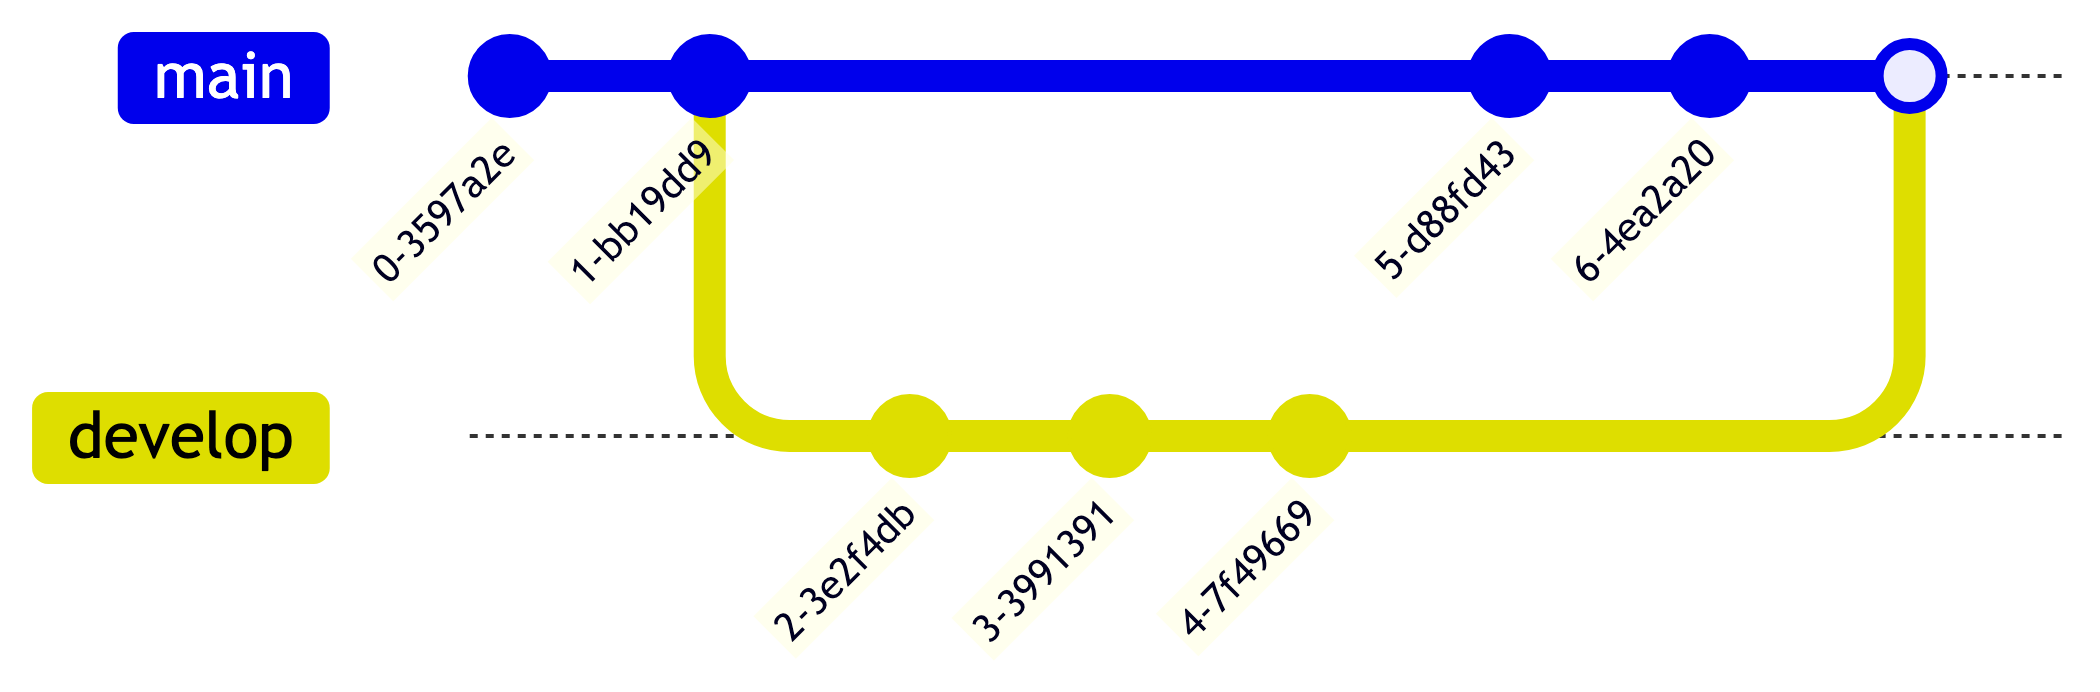
\includegraphics[width=5.47in,height=1.8in]{chapters/ru/_debug/debug_files/figure-latex/mermaid-figure-2.png}

\section{Картинки}\label{debug-pics}

\begin{figure}

\centering{

\centering{

\pandocbounded{
\includegraphics[keepaspectratio]{chapters/ru/_debug/img/debug-pic.jpg}}

}

\subcaption{\label{fig-debug-1}Первая картинка}

\centering{

\pandocbounded{
\includegraphics[keepaspectratio]{chapters/ru/_debug/img/debug-pic.jpg}}

}

\subcaption{\label{fig-debug-2}Вторая картинка}

}

\caption{\label{fig-debug}Дебажные картинки в~обычном лэйауте}

\end{figure}%

\begin{figure}

\begin{minipage}{0.50\linewidth}

\centering{

\pandocbounded{
\includegraphics[keepaspectratio]{chapters/ru/_debug/img/debug-pic.jpg}}

}

\subcaption{\label{fig-debug-1}Левая картинка}

\end{minipage}%
%
\begin{minipage}{0.50\linewidth}

\centering{

\pandocbounded{
\includegraphics[keepaspectratio]{chapters/ru/_debug/img/debug-pic.jpg}}

}

\subcaption{\label{fig-debug-2}Правая картинка}

\end{minipage}%

\caption{\label{fig-debug}Дебажные картинки в~ лэйауте на~2 колонки}

\end{figure}%

\phantomsection\label{refs}
\begin{CSLReferences}{1}{0}
\bibitem[\citeproctext]{ref-knuth84}
Knuth, Donald E. 1984. {«Literate Programming»}. \emph{Comput. J.} 27
(2): 97--111. \url{https://doi.org/10.1093/comjnl/27.2.97}.

\end{CSLReferences}




\end{document}
